\begin{frame}
  \frametitle{}
  \begin{quote}
    Но тем не менее число исследователей в этом направлении весьма ограничено, и в сущности винтовое исчисление продолжает оставаться неизвестным громадному кругу лиц, занимающихся механикой твердого тела и сплошной среды, а тем более инженерам, работающим в промышленности.
  \end{quote}
  \fullcite[14]{Dimentberg:1965}
\end{frame}

%%--------------------------
\begin{frame}
  \frametitle{Момент вектора}
  \begin{columns}
    \begin{column}{0.3\textwidth}
      \begin{center}
        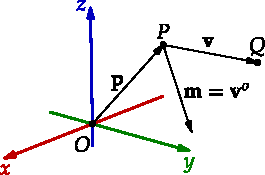
\includegraphics{img/screws/moment01}
      \end{center}
    \end{column}
    \begin{column}{0.7\textwidth}
      \emph{Моментом} вектора $\vb{v}$ относительно начала координат $O$ называется вектор
      \begin{equation*}
        \vb{m} = \vb{p} \times \vb{v},
      \end{equation*}
      где $\vb{p}$ — радиус вектор точки $P$. Момент зависит от точки $O$, поэтому также обозначают $\vb{m} = \vb{v}^{o}$.
      \begin{itemize}
        \item Точка $O$ — точка начала отсчета или \emph{точка приведения}.
        \item В силу свойств векторного произведения:
        \begin{equation*}
          \vb{m} \perp (OPQ),
        \end{equation*}
        \begin{equation*}
          \norm{\vb{m}} = 2S_{\triangle OPQ},
        \end{equation*}
        \item В общем случае $\vb{p}$ не перпендикулярен $\vb{v}$.
        \item Два равных вектора называются \emph{эквивалентными}, если их моменты равны.
        \item \emph{Скользящие векторы} — равные векторы, лежащие на одной прямой.
      \end{itemize}
    \end{column}
  \end{columns}
\end{frame}

%%--------------------------
\begin{frame}
  \frametitle{Скользящий вектор}
  \begin{columns}
    \begin{column}{0.4\textwidth}
      \begin{center}
        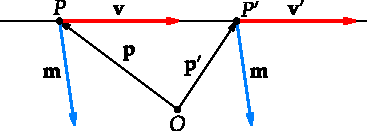
\includegraphics{img/screws/moment02}
      \end{center}
    \end{column}
    \begin{column}{0.6\textwidth}
      Если $\vb{v}$ — направляющий вектор прямой, то его момент $\vb{m}$ одинаков для любой точки $P$ данной прямой. Если $\vb{p}^{\prime} = \vb{p} + \Delta \vb{v}$, то
      \begin{equation*}
        \vb{m}^{\prime} = \vb{p}^{\prime} \times \vb{v} = (\vb{p} + \Delta \vb{v})\times \vb{v} = \vb{p} \times \vb{v} + \Delta \vb{v} \times \vb{v} = \vb{p} \times \vb{v} = \vb{m}.
      \end{equation*}
      Скользящие векторы таким образом являются одновременно и эквивалентными.
      Для скользящих векторов:
        \begin{equation*}
          (\vb{v}, \vb{m}) = 0.
        \end{equation*}
    \end{column}
  \end{columns}
  Примеры скользящих векторов:
  \begin{itemize}
    \item угловая скорость;
    \item вектор силы;
    \item направляющий вектор прямой.
  \end{itemize}
  Угловая скорость — векторная величина, задающая мгновенную ось вращения абсолютно твердого тела, то есть в геометрическом смысле — направляющий вектор прямой, представляющей ось вращения.
\end{frame}

%%--------------------------
\begin{frame}
  \frametitle{Замена начала координат}
  \begin{columns}
    \begin{column}{0.5\textwidth}
      \begin{center}
        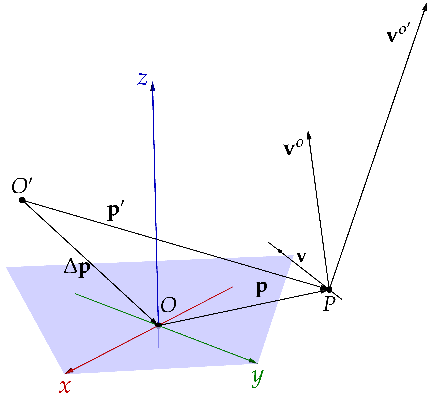
\includegraphics[height=0.9\textheight]{img/screws/moment03}
      \end{center}
    \end{column}
    \begin{column}{0.5\textwidth}
      Произведем замену начала координат $O \to O^{\prime}$. Вектор $\vb{v}$ не измениться, так как он свободный. Если $\Delta \vb{p} = \vb{O^\prime O}$, то $\vb{p}^{\prime} = \vb{p} + \Delta \vb{p}$, тогда
      \begin{equation*}
        \vb{v}^{o^\prime} = \vb{p}^\prime \times \vb{v} = (\vb{p} + \Delta \vb{p}) \times \vb{v} = \vb{p} \times \vb{v} + \Delta \vb{p} \times \vb{v} = \vb{v}^{o} + \Delta\vb{p}\times \vb{v},
      \end{equation*}
      \begin{equation*}
        \vb{v}^{o^\prime} = \vb{v}^{o} + \Delta\vb{p}\times \vb{v}
        \text{ или }
        \vb{m}^{\prime} = \vb{m} + \Delta\vb{p}\times \vb{v}.
      \end{equation*}
      Вычислим скалярное произведение:
      \begin{equation*}
        (\vb{v}, \vb{v}^{o^\prime}) = (\vb{v}, \vb{v}^{o} + \Delta \vb{p} \times \vb{v}) = (\vb{v}, \vb{v}^{o}),
      \end{equation*}
      в силу $\vb{v} \perp \Delta \vb{p}\times \vb{v}$.
      
      Скалярное произведение $(\vb{v}, \vb{v}^{o})$ — \emph{скалярный инвариант}, так как не зависит от выбора начала координат.
    \end{column}
  \end{columns}
\end{frame}

%%--------------------------
\begin{frame}
  \frametitle{М\'отор и винт}
  \emph{М\'отором} (\textbf{мо}мент + век\textbf{тор}) назовем двойку векторов $\{\vb{v} \mid \vb{v}^{o}\}$, где:
  \begin{itemize}
    \item $\vb{v}$ — скользящий вектор (направляющий вектор прямой), \emph{главная часть},
    \item $\vb{v}^{o}$ — его момент относительно начала координат $O$ — \emph{моментная часть}.
  \end{itemize}
  Оба вектора откладываются от произвольной точки $P$ прямой с радиус вектором $\vb{p}$ и $\vb{v}^{o} = \vb{p} \times \vb{v}$.

  Мотор можно также записать в виде \emph{дуального вектора} или \emph{диады}:
  \begin{equation*}
    \vb{R} = \vb{v} + \varepsilon\vb{v}^{o}, \;\;
    \varepsilon^2 = 0, \;\; \varepsilon \not = 0,
  \end{equation*}
  где $\varepsilon$ — дуальная мнимая единица (мнимая единица комплексных чисел параболического типа) или символ комплексности Клиффорда.

  \emph{Винтом} называют мотор, у которого $\vb{v} \parallel \vb{v}^{o}$. Любой мотор можно превратить в винт путем замены начала координат $O$. Прямая $l$ для которой $\vb{v}$ является направляющей, называется \emph{осью винта}.

  Если $\vb{v} \parallel \vb{v}^{o}$, то $\vb{v}^{o} = p \vb{v}$, где $p$ — \emph{параметр винта} (действительное число).
\end{frame}

%%--------------------------
\begin{frame}
  \frametitle{Замена мотора на винт}
  \begin{columns}
    \begin{column}{0.35\textwidth}
      \begin{center}
        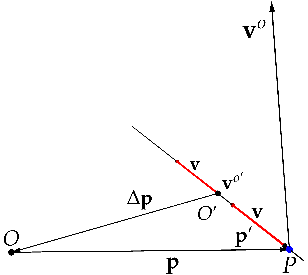
\includegraphics{img/screws/moment04}
      \end{center}
    \end{column}
    \begin{column}{0.65\textwidth}
      Пусть дан мотор
      \begin{equation*}
        \vb{R} = \vb{v} + \vb{v}^{o}\varepsilon, \;\; \vb{v} \not \parallel \vb{v}^{o}.
      \end{equation*}
      Заменим начало координат $O \to O^{\prime}$, $O^\prime \in l$, где $l$ — прямая, для которой $\vb{v}$ направляющий вектор. Причем возьмем
      \begin{equation*}
        \vb{O^{\prime}O} = 
        \dfrac{\vb{v}^{o}\times \vb{v}}{\norm{\vb{v}}^2}.
      \end{equation*}
      Можно показать, что такая замена приведет к тому, что
      \begin{equation*}
        \vb{v}^{o^{\prime}} = \dfrac{(\vb{v}, \vb{v}^{o})}{\norm{\vb{v}}^2}\vb{v} = p\vb{v},
        \quad
        p = \dfrac{(\vb{v}, \vb{v}^o)}{\norm{\vb{v}}^2}.
      \end{equation*}
      В случае скользящего вектора:
      \begin{itemize}
        \item $\vb{v}^{o^{\prime}} = \vb{0}$ и $p = 0$;
        \item точка $O^\prime$ — ближайшая точка прямой $l$ к началу координат $O$ или проекция $O$ на $l$;
        \item $\vb{OO}^{\prime} = \dfrac{\vb{v} \times \vb{v}^o}{\norm{\vb{v}}^2}$.
      \end{itemize}
    \end{column}
  \end{columns}
\end{frame}

%%--------------------------
\begin{frame}
  \frametitle{Единичный винт, нуль-система, координаты Плюккера}
  \begin{columns}
    \begin{column}{0.5\textwidth}
      \begin{center}
        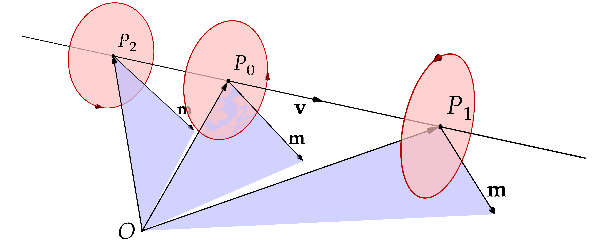
\includegraphics[width=1.0\textwidth]{img/screws/plucker}
      \end{center}
    \end{column}
    \begin{column}{0.5\textwidth}
      \emph{Единичным} называется винт с нулевым параметром $p$ и с единичным вектором $\vb{e}$. Единичному винту соответствует мотор
      \begin{equation*}
        \vb{E} = \vb{e} + \vb{e}^{o}\varepsilon,
        \quad
        (\vb{e}, \vb{e}^o) = 0 = p,
        \quad
        \norm{\vb{v}} = 1.
      \end{equation*}
      Всякий единичный винт геометрически можно интерпретировать как прямую, на которой заданно направление по правилу буравчика (отсюда название винт).

      Условие $(\vb{e}, \vb{e}^o) = 0$ — \emph{условие Плюккера}. Все моторы и винты, для которых оно выполняется, задают прямые в трехмерном пространстве.
    \end{column}
  \end{columns}

  \begin{block}{Однородное представление прямой}
    Вообще, из любой пары векторов $\{\vb{v} \mid \vb{m}\}$ для которых $(\vb{v}, \vb{m}) = 0$ можно составить диаду $\vb{L} = \vb{v} + \varepsilon \vb{m}$ и однозначно интерпретировать ее как прямую, проходящую через точку с радиус вектором $\vb{p} = \vb{v} \times \vb{m}$ по направлению $\vb{v}$. Шесть компонент (три от $\vb{v}$ и три от $\vb{m}$) называются \emph{координатами Плюккера} или нуль-системой~\cite{KleinHoherGeometrie}.
  \end{block}
\end{frame}

%%--------------------------
\begin{frame}
  \frametitle{Дуальный угол}
  \begin{columns}
    \begin{column}{0.4\textwidth}
      \begin{center}
        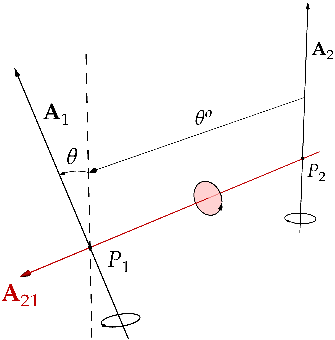
\includegraphics{img/screws/moment05}
      \end{center}
    \end{column}
    \begin{column}{0.6\textwidth}
      \emph{Дуальным углом} $\Theta = \theta + \theta^{o}\varepsilon$ между двумя винтами $\vb{A}_1$ и $\vb{A}_2$ называется фигура, образованная осями этих винтов и отрезком прямой $P_2P_1$, пересекающей эти оси под прямым углом.
      \begin{itemize}
        \item Винт $\vb{A}_{21}$ с осью в виде прямой $(P_2P_1)$ — \emph{ось дуального угла}.
        \item Дуальная часть угла $\theta^{o} = \norm{\vb{P_2P_1}}$.
        \item Действительная часть угла $\theta = \measuredangle (\vb{A}_2, \vb{A}_1)$.
      \end{itemize}
      Дуальный угол $\Theta$ определяется винтом
      \begin{equation*}
        \vb{\Theta} = \Theta \vb{A}_{21} = (\theta + \theta^{o}\varepsilon)\vb{A}_{21}.
      \end{equation*}

      Для вычисления тригонометрических функций от дуального угла используются следующие формулы:
      \begin{align*}
        &\sin \Theta = \sin (\theta + \theta^{o}\varepsilon) = \sin \theta + \theta^{o} \cos\theta \varepsilon,\\
        &\cos \Theta = \cos (\theta + \theta^{o}\varepsilon) = \cos\theta - \theta^{o} \sin\theta \varepsilon,\\
        &\tg \Theta = \tg (\theta + \theta^{o}\varepsilon) = \tg \theta + \dfrac{\theta^o}{\cos^2\theta}\varepsilon.
      \end{align*}
    \end{column}
  \end{columns}
\end{frame}

%%--------------------------
\begin{frame}
  \frametitle{Скалярное умножение винтов}
  Пусть даны два винта $\vb{R}_1 = \vb{r}_1 + \vb{r}^{o}_1 \varepsilon$ и $\vb{R}_2 = \vb{r}_2 + \vb{r}^{o}_2 \varepsilon$. Их скалярное произведение вычисляется по формуле:
  \begin{equation*}
    \boxed{
    (\vb{R}_1, \vb{R}_2) = (\vb{r}_1, \vb{r}_2) + [(\vb{r}_1, \vb{r}_{2}^{o}) + (\vb{r}^{o}_1, \vb{r}_2)]\varepsilon
    }
  \end{equation*}
  Величина $M(\vb{R}_1, \vb{R}_2) = (\vb{r}_1, \vb{r}_{2}^{o}) + (\vb{r}^{o}_1, \vb{r}_2)$ — \emph{взаимный момент} двух винтов (двух прямых).
  \begin{itemize}
    \item Если $M \not = 0$, то оси винтов (прямые) скрещиваются и
    \begin{itemize}
      \item если $M > 0$, то поворот от $\vb{R}_1$ к $\vb{R}_2$ — правый,
      \item если $M < 0$, то поворот от $\vb{R}_1$ к $\vb{R}_2$ — левый.
    \end{itemize}
    \item Если $M = 0$, то оси винтов лежат в одной плоскости (компланарны).
  \end{itemize}
  Зная формулу для скалярного произведения, можно определить квадрат нормы винта $\vb{R} = \vb{r} + \vb{r}^o\varepsilon$ как
  \begin{equation*}
    \norm{\vb{R}}^2 = (\vb{R}, \vb{R}) = (\vb{r}, \vb{r}) + 2(\vb{r}, \vb{r}^o)\varepsilon = \norm{\vb{r}}^2 + 2(\vb{r}, \vb{r}^o)\varepsilon.
  \end{equation*}
  Используя формулу $\sqrt{a + b\varepsilon} = \sqrt{a} + \dfrac{b}{2\sqrt{a}}\varepsilon$ можно также вычислить
  \begin{equation*}
    \norm{\vb{R}} = \sqrt{(\vb{R}, \vb{R})} = \norm{\vb{r}}(1 + p\varepsilon),
    \;\;
    \text{где }
    p = \dfrac{(\vb{r}, \vb{r}^o)}{\norm{\vb{r}}^2}.
  \end{equation*}
  Для единичного винта параметр $p = 0$, так как по условию Плюккера $(\vb{r}, \vb{r}^o) = 0$ и норма винта --- действительное число.
\end{frame}

%%--------------------------
\begin{frame}
  \frametitle{Вычисление скалярного произведения через дуальный угол}
  \begin{columns}
    \begin{column}{0.4\textwidth}
      \begin{center}
        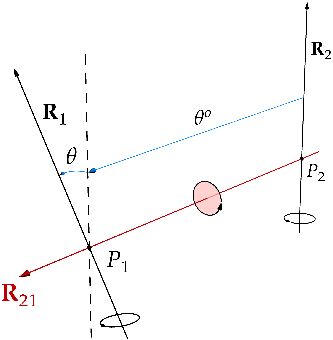
\includegraphics{img/screws/moment06}
      \end{center}
    \end{column}
    \begin{column}{0.6\textwidth}
      Если даны два винта $\vb{R}_1$ и $\vb{R}_2$:
      \begin{equation*}
        \vb{R}_1 = \vb{r}_1 + \vb{r}^{o}_1 \varepsilon,\;\;
        \vb{R}_2 = \vb{r}_2 + \vb{r}^{o}_2 \varepsilon
      \end{equation*}
      и дуальный угол между их осями $\Theta = \theta + \theta^{o}\varepsilon$, то можно доказать, что скалярное произведение этих винтов вычисляется также по формуле:
      \begin{equation*}
        (\vb{R}_1, \vb{R}_2) = \norm{\vb{R}_1} \norm{\vb{R}_2} \cos \Theta 
      \end{equation*}
      где
      \begin{equation*}
        \cos \Theta = \cos (\theta + \theta^{o}\varepsilon) = \cos\theta - \theta^{o} \sin\theta \varepsilon.
      \end{equation*}
      Подробное доказательство см. в~\cite[46]{Dimentberg:1965} и его сокращенный вариант в книге~\cite[55]{Chelnokov:2006}.
    \end{column}
  \end{columns}
\end{frame}

%%--------------------------
\begin{frame}
  \frametitle{Винтовое (векторное) умножение винтов}
  Пусть даны два винта $\vb{R}_1 = \vb{r}_1 + \vb{r}^{o}_1 \varepsilon$ и $\vb{R}_2 = \vb{r}_2 + \vb{r}^{o}_2 \varepsilon$. Их винтовое (векторное) произведение вычисляется по формуле:
  \begin{equation*}
    \boxed{
    \vb{R}_1 \times \vb{R}_2 = 
    \vb{r}_1 \times \vb{r}_2 + (\vb{r}_1 \times \vb{r}^{o}_2 + \vb{r}^{o}_1 \times \vb{r}_2)\varepsilon
    }
  \end{equation*}
  Аналогично можно доказать, что
  \begin{equation*}
    \vb{R}_1 \times \vb{R}_2 = \norm{\vb{R}_1}\norm{\vb{R}_2}\sin\Theta \vb{R}_{21},
  \end{equation*}
  где $\Theta$ — дуальный угол, $\vb{R}_{21}$ — ось дуального угла.
\end{frame}

%%--------------------------
\begin{frame}
  \frametitle{Дуальные координаты винта}
  Рассмотрим диаду $\vb{R} = \vb{r} + \vb{r}^{o}\varepsilon$ и запишем ее в компонентном виде:
  \begin{equation*}
    \vb{R} = 
    \begin{bmatrix}
      x\\y\\z
    \end{bmatrix}
    +
    \begin{bmatrix}
      x^o\\y^o\\z^o
    \end{bmatrix}
    \varepsilon
    =
    \begin{bmatrix}
      x + x^o\varepsilon\\
      y + y^o\varepsilon\\
      z + z^o\varepsilon
    \end{bmatrix}
    =
    \begin{bmatrix}
      R_x\\R_y\\R_z
    \end{bmatrix}
  \end{equation*}
  где $R_x, R_y, R_z$ — дуальные числа. Таким образом винт можно представить двумя способами:
  \begin{itemize}
    \item шестью действительными числами (координатами Плюккера) в виде компонент двух векторов $\{\vb{r} \mid \vb{r}^o\}$;
    \item тремя дуальными числами — \emph{дуальными координатами винта}.
  \end{itemize}
  Если ввести три дуальных угла $\Alpha = \alpha + \alpha^o\varepsilon$, $\Beta = \beta + \beta^o\varepsilon$, $\Gamma = \gamma + \gamma^o\varepsilon$, которые образуются осью винта с осями декартовой системы координат $Ox$, $Oy$ и $Oz$, то компоненты винта можно представить также как
  \begin{equation*}
    \vb{R} = 
    R
    \begin{bmatrix}
      \cos\Alpha\\ 
      \cos\Beta\\ 
      \cos\Gamma\\ 
    \end{bmatrix}
    \quad
    R = \norm{\vb{R}}.
  \end{equation*}
  Косинусы от $\Alpha, \Beta, \Gamma$ — аналоги направляющих косинусов для случая обычных векторов.
\end{frame}

%%--------------------------
\begin{frame}
  \frametitle{Условие единичности винта}
  Запишем винт в дуальных компонентах. Если условится дуальные числа обозначать прописными буквами, то можно записать:
  \begin{equation*}
    \vb{R} = 
    \begin{bmatrix}
      X\\Y\\Z
    \end{bmatrix}
    =
    \begin{bmatrix}
      x + x^o\varepsilon\\
      y + y^o\varepsilon\\
      z + z^o\varepsilon
    \end{bmatrix}
    =
    \begin{bmatrix}
      R\cos\Alpha\\
      R\cos\Beta\\
      R\cos\Gamma
    \end{bmatrix}
  \end{equation*}
  Квадрат нормы винта $\vb{R}$ вычисляется следующим образом:
  \begin{multline*}
    (\vb{R}, \vb{R}) = (\vb{r}, \vb{r}) + (\vb{r}, \vb{r}^o) \varepsilon = x^2 + y^2 + z^2 + 2(xx^o + y y^o + z z^o)\varepsilon = {} \\
    {} = \big(x^2 + 2xx^o\varepsilon\big) + \big(y^2 + 2yy^o\varepsilon\big) + \big(y^2 + 2yy^o\varepsilon\big) = X^2 + Y^2 + Z^2 = R (\cos^2\Alpha + \cos \Beta + \cos \Gamma) = R = \norm{\vb{R}},
  \end{multline*}
  что согласуется с формулой для квадрата дуального числа $(a + b\varepsilon)^2 = a^2 + 2ab\varepsilon$. Также получаем, что
  \begin{equation*}
    \cos^2\Alpha + \cos \Beta + \cos \Gamma = 1.
  \end{equation*}
  Если $\vb{E} = \vb{e} + \vb{e}^o\varepsilon = (X, Y, Z)^T$ — единичный винт, то из условия единичности $\norm{\vb{E}} = 1$ следует:
  \begin{equation*}
    (\vb{E}, \vb{E}) = 1 = x^2 + y^2 + z^2 + 2(xx^o + y y^o + z z^o)\varepsilon,
  \end{equation*}
  что приводит к $x^2 + y^2 + z^2 = 1 = \norm{\vb{e}}$ и условию Плюккера:
  \begin{equation*}
    (\vb{e}, \vb{e}^o) = xx^o + y y^o + z z^o = 0.
  \end{equation*}
\end{frame}

%%--------------------------
\begin{frame}
  \frametitle{Скалярное и винтовое произведения в дуальных координатах}
  Можно доказать, что для двух винтов $\vb{R}_1 = (X_1, Y_1, Z_1)^T$ и $\vb{R}_2 = (X_2, Y_2, Z_2)^T$ справедливо:
  \begin{equation*}
    (\vb{R}_1, \vb{R}_2) = X_1X_2 + Y_1Y_2 + Z_1Z_2,
    \qquad
    \vb{R}_1 \times \vb{R}_2 = 
    \begin{vmatrix}
      \vb{i} & \vb{j} & \vb{k}\\
      X_1 & Y_1 & Z_1\\
      X_2 & Y_2 & Z_2\\
    \end{vmatrix}
  \end{equation*}
  где $\vb{i}, \vb{j}, \vb{k}$ — базисные векторы декартовой системы координат.

  Для скалярного произведения также запишем:
  \begin{equation*}
    (\vb{R}_1, \vb{R}_2) = x_1x_2 + y_1y_2 + z_1 z_2 + (x_1x^o_2 + x_1^ox_2 + y_1y_2^o + y_1^oy_2 + z_1z^o_2 + z_1^oz_2)\varepsilon,
  \end{equation*}
  где $M(\vb{R}_1, \vb{R}_2) = x_1x^o_2 + x_1^ox_2 + y_1y_2^o + y_1^oy_2 + z_1z^o_2 + z_1^oz_2$ — взаимный момент двух винтов.
\end{frame}

%%--------------------------
\begin{frame}
  \frametitle{Сводка формул}

  \begin{center}
    \begin{tblr}{
        rowspec={Q[c, m]},
        hlines = {0.25pt,dashed},
        hline{1-2} = {1pt,solid},
        vlines = {0.25pt,solid}
      }
      \textbf{Векторная запись} & \textbf{Дуальная запись}\\
      $
        \vb{R} = \vb{r} + \vb{r}^{o} \varepsilon = 
        \begin{bmatrix}
          x\\y\\z
        \end{bmatrix}
        +
        \varepsilon
        \begin{bmatrix}
          x^o\\y^o\\z^o
        \end{bmatrix}
      $
      &
      $
        \vb{R} = 
        \begin{bmatrix}
          x + x^o\varepsilon\\
          y + y^o\varepsilon\\
          z + z^o\varepsilon
        \end{bmatrix}
        =
        \begin{bmatrix}
          X\\Y\\Z
        \end{bmatrix}
      $
      \\
      {
        $(\vb{R}_1, \vb{R}_2) = (\vb{r}_1, \vb{r}_2) + [(\vb{r}_1, \vb{r}_{2}^{o}) + (\vb{r}^{o}_1, \vb{r}_2)]\varepsilon$\\
        $(\vb{R}_1, \vb{R}_2) = \norm{\vb{R}_1} \norm{\vb{R}_2} \cos \Theta$
      }
      &
      $(\vb{R}_1, \vb{R}_2) = X_1X_2 + Y_1Y_2 + Z_1Z_2$\\
      {
        $\vb{R}_1 \times \vb{R}_2 = \vb{r}_1 \times \vb{r}_2 + (\vb{r}_1 \times \vb{r}^{o}_2 + \vb{r}^{o}_1 \times \vb{r}_2)\varepsilon$
        \\
        $\vb{R}_1 \times \vb{R}_2 = \norm{\vb{R}_1}\norm{\vb{R}_2}\sin\Theta \vb{R}_{21}$
      }
      &
      $
        \vb{R}_1 \times \vb{R}_2 = 
        \begin{vmatrix}
          \vb{i} & \vb{j} & \vb{k}\\
          X_1 & Y_1 & Z_1\\
          X_2 & Y_2 & Z_2\\
        \end{vmatrix}
      $\\
    \end{tblr}
  \end{center}
  
\end{frame}